\section{Proposed RLC Fast\\ Retransmission}\label{sec:eval}

% Four case
\begin{figure*}[th!]
	\centering
	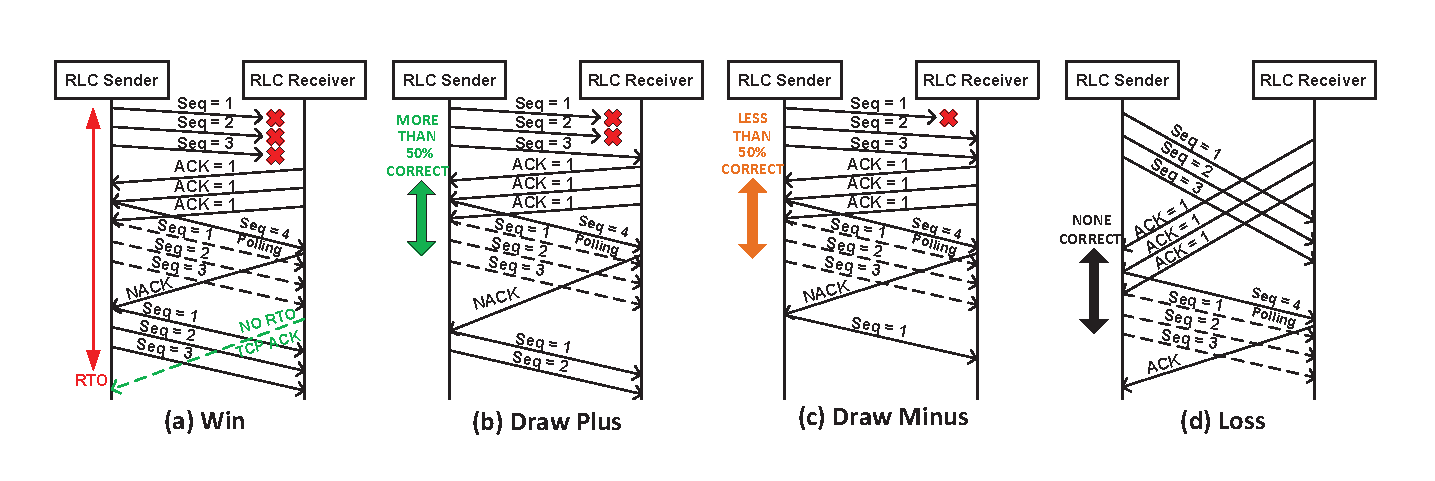
\includegraphics[width=\textwidth]{figs/cost_benefit.eps}
	\vspace{-4ex}
%	\subfigure[Win]{
%		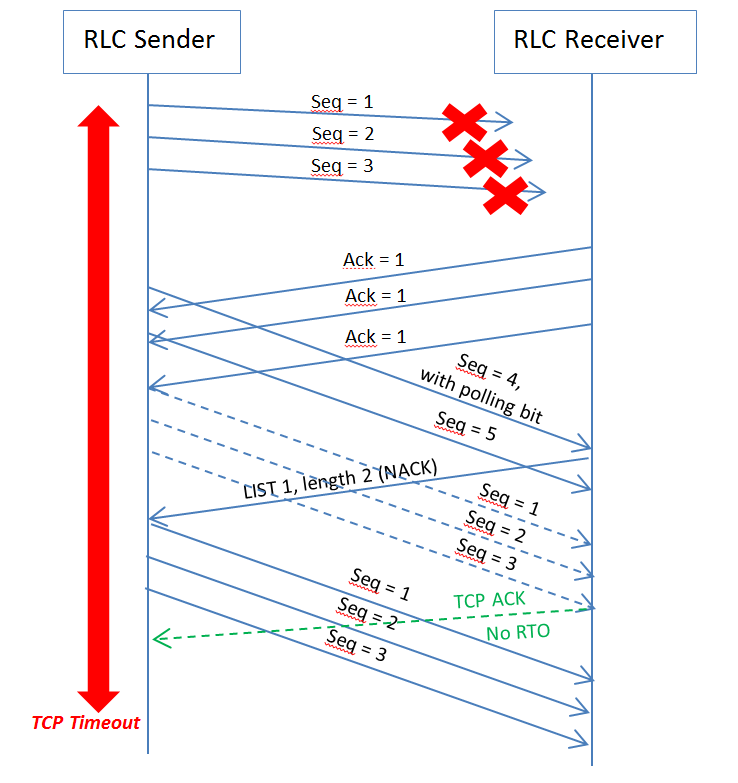
\includegraphics[width=0.35\textwidth]{figs/Win.png}
%		\label{fig:win}
%	}
%	~~~
%	\subfigure[Draw Plus]{
%		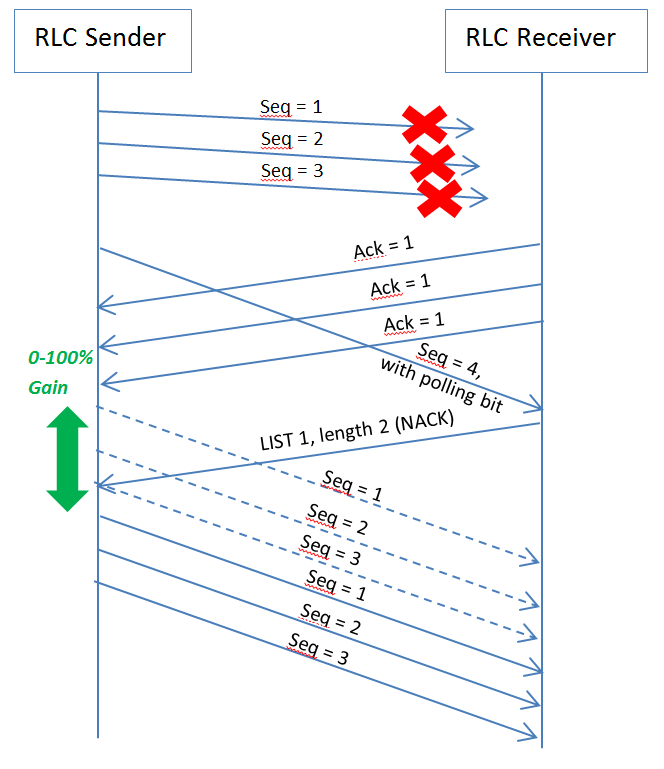
\includegraphics[width=0.35\textwidth]{figs/Draw_plus.png}
%		\label{fig:draw.plus}
%	}
%	\\
%	\subfigure[Draw Minus]{
%		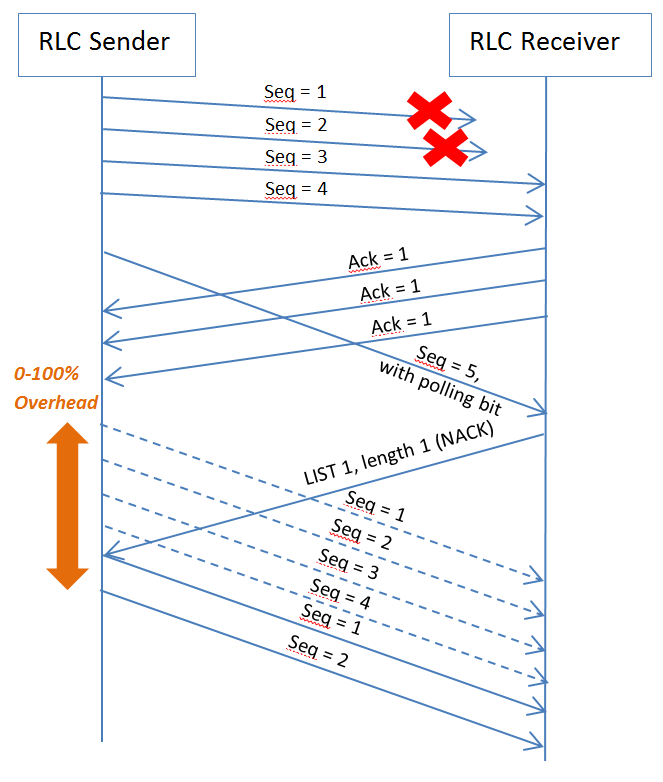
\includegraphics[width=0.35\textwidth]{figs/Draw.png}
%		\label{fig:draw.minus}
%	}
%	~~~
%	\subfigure[Loss]{
%		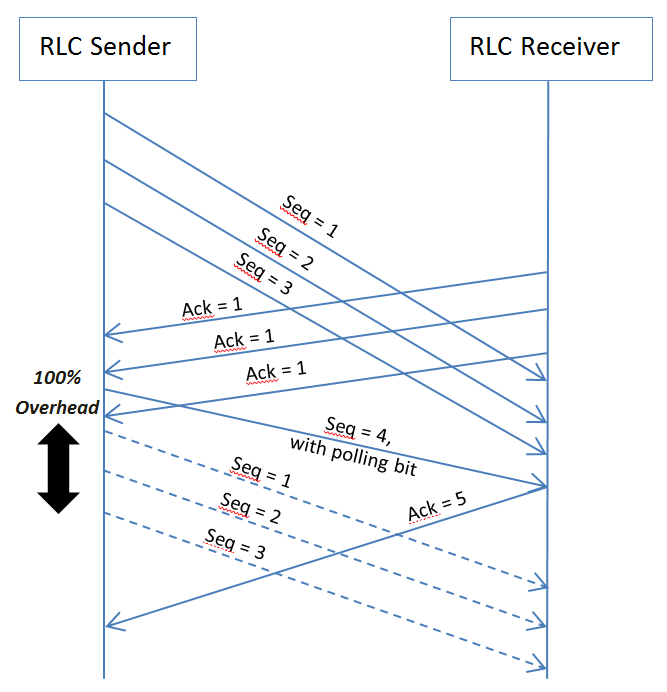
\includegraphics[width=0.35\textwidth]{figs/Loss.png}
%		\label{fig:loss}
%	}
	\ncaption{\textit{Win}: RLC Fast Re-Tx avoids a TCP RTO. \textit{Draw Plus}: Prediction accuracy is more than 50\%. \textit{Draw Minus}: Prediction accuracy is less than 50\%. \textit{Loss}: All predictions are wrong.}
	\label{fig:cost.benefit.detail}
\end{figure*}

As we have shown in \S\ref{sec:qxdm.analysis}, negative interactions between RLC-level retransmissions and TCP-level retransmissions result in increased delay. In this section, we propose a mechanism for reducing this delay by implementing RLC fast retransmission to allow the RLC layer to respond faster to packet loss.
%\subsection{RLC Fast Retransmission}

%\subsection{RTT Estimation}
First, we explain how we measure RTTs in the RLC layer.  As STATUS PDUs (ACK or NACK) are not generated by every received PDU, and are only triggered if a polling request is received or one or more PDUs are missing in the receiver buffer~\cite{spec-3G-RLC}, it is difficult to estimate RTTs directly.  QxDM traces only include client-side information, so we have no data on when the server receives each PDU.  We estimate the RTTs of RLC PDUs based on the timestamp difference between the most recent sender polling request and the most recently received ACK.  The RLC configuration limits the maximum polling request frequency to 500ms.  A previous mobile RTT estimation study shows that the autocorrelation coefficient between two RTT measurements within 500 ms is more than 0.6~\cite{proteus}, so this estimate is reasonable.

%We first define the RTT in RLC layer. In the RLC protocol, the STATUS PDUs (ACK or NACK) don't generate by every received RLC PDU, but triggered either by receiving a polling request from the sender or by detecting one or more missed PDUs from its receiver buffer~\cite{spec-3G-RLC}. Since the QxDM traces are collected at the client side, we don't have the information of when the server side receive the PDU. Thus, I estimate the RTT of a RLC PDU based on the timestamp difference between the most recent sender's polling request and received ACK. Based on RLC configuration, the maximum polling request frequency is 500 ms. One of the previous mobile RTT estimation study shows the autocorrelation coefficient of two RTT measurements within 500 ms is more than 0.6~\cite{proteus}. Therefore, my estimation is still reasonable to be considered as the real RLC RTT value.

\subsection{Cost-Benefit Analysis}

% \mycomment{I'm not quite sure what is meant.  If they would have been retransmitted in the future anyway?}
% \mycomment{Is this part necessary given that we apparently consider four other cases instead?}
% To evaluate this new promosed mechanism, we perform a cost-benefit analysis over our existing QxDM trace.  For the PDUs resent through fast retransmission, we determine if they are transmitted in the future  then we subtract the RTT value that would occur with fast retransmit with the RTT value from the trace.  If the difference is less than zero, we count it as a benefit; otherwise it is a cost. 

To evaluate the proposed \textit{Fast Re-Tx} mechanism, we perform a cost-benefit analysis using the \emph{QxDM\_{}UDP\_{}Trace} and \emph{QxDM\_{}TCP\_{}Trace}. In our proposal, when the sender receives 3 duplicate ACKs, the device predicts that all the previous unacknowledged PDUs have not been received by the receiver, and transmits all of them right away. However, there is a chance that the PDUs are actually delayed by radio channel contention. We validate the actual cause of the delays using the QxDM traces, based on whether the sender receives an ACK or a NACK after the \textit{Fast Re-Tx} occurs. A future ACK implies all the PDUs are delayed over the channel, while a NACK could indicate the PDUs are lost~\cite{spec-3G-RLC}.

To perform the cost/benefit analysis, we categorize all duplicate ACK scenarios into 4 cases based on the prediction accuracy, which is the ratio of the number of PDU divided by the total number of \textit{Fast Re-Tx} PDU. We call them --- Win, Draw\_{}Plus, Draw\_{}Minus, and Loss.  Draw\_{}Plus occurs when the sender receives a NACK and more than 50\% of the PDUs sent in \textit{Fast Re-Tx} would have to be retransmitted anyway (according to the traces.
)
This is illustrated in Figure~\ref{fig:cost.benefit.detail}(b) --- there is a decrease in latency.  The ``win" case is similar, but occurs where the TCP RTO was avoided entirely, leading to further latency reductions as shown in Figure~\ref{fig:cost.benefit.detail}(a).  ``Draw\_{}Minus" occurs when less than 50\% of the PDUs retransmitted through our proposed mechanism would have been retransmitted anyway --- unnecessary retransmissions have occurred. This case is shown in Figure~\ref{fig:cost.benefit.detail}(c). If all PDUs were successfully delivered to the receiver, we refer to this case as ``Loss",  as shown in Figure\ref{fig:cost.benefit.detail}(d). Redundant data was transmitted and there were no latency gains.
%To explicitly analyze the cost/benefit behavior, we categorize all the duplicate ACK scenarios into 4 cases, which we call \textbf{Win}, \textbf{Draw\_{}Plus}, \textbf{Draw\_{}Minus} and \textbf{Loss}.  \textbf{Draw\_{}Plus} occurs when the sender receives a NACK and more than 50\% of the PDUs that would be sent in fast-retransmit were retransmitted in the real trace. This can be seen in Figure~\ref{fig:cost.benefit.detail}(b) --- the decrease in RTT is beneficial. \textbf{Win} is similar, but occurs where the TCP RTO would have been avoided entirely leading to further latency reductions as in Figure~\ref{fig:cost.benefit.detail}(a). \textbf{Draw\_{}Minus} occurs when less than 50\% of the PDUs retransmitted through our proposed mechanism were retransmitted in the actual trace. This case is shown in Figure~\ref{fig:cost.benefit.detail}(c). If all PDUs were successfully delivered to the receiver, we refer to this case as \textbf{Loss} as in Figure\ref{fig:cost.benefit.detail}(d) redundant data was transmitted and there were no latency gains.

%In order to know whether the new proposed RLC mechanism works, I apply a cost-benefit analysis over the existing \emph{QxDM\_{}Trace}. The definition of benefit and cost is straight forward. Basically, if the fast retransmitted PDUs will be transmitted in the future, then we compare the RTT if it transmitted right after the duplicate ACKs with the real RTT value in the trace. If the difference is less than 0, we call that is a benefit. In the same way, if it is greater than 0, we call it a cost. However, we want to know if the PDU is really lost over the channel, or it just gets delayed due to channel contention. That depends on whether the sender receives a ACK or NACK (a list of unreceived PDU sequence numbers). We categorize the situations into four cases -- Win, Draw\_{}Plus, Draw\_{}Minus, and Loss. If the sender will receive a NACK, and more than 50\% of the fast retransmitted PDUs will retransmit in the real trace, then we call the case "Draw\_{}Plus" as in Figure~\ref{fig:draw.plus}. Since it would brings us benefit if the fast retransmit RTT is less than the RTT in the real trace. The "Win" case is defined that if we could avoid a TCP RTO based on the "Draw\_{}Plus" in Figure~\ref{fig:win}. In that case, RLC layer benefit is the same as "Draw\_{}Plus", but I want to highlight that it could bring further latency benefit over the transport layer. "Draw\_{}Minus" occurs when less than 50\% of the fast retransmitted PDUs get really retransmitted in the real trace as in Figure~\ref{fig:draw.minus}. If the sender gets a ACK with a larger sequence number, then all the PDUs were successfully delivered to the receiver. In that case, we called the case "Loss", since all the retransmitted packets are redundant as in Figure~\ref{fig:loss}. To summarize all four cases:
%
%\begin{itemize}
%\item \textbf{Win:} A special case of Draw\_{}Plus with extra benefit of avoid TCP RTO.
%\item \textbf{Draw\_{}Plus:} More than half of the fast retransmitted packets really retransmitted in the real trace.
%\item \textbf{Draw\_{}Minus:} Less than half of the fast retransmitted packets really retransmitted in the real trace.
%\item \textbf{Loss:} None of the fast retransmitted packets retransmitted in the real trace.
%\end{itemize}

As we can see from Table~\ref{tab:rlc.fast.sim}, almost exactly 75\% of the time there would be a clear benefit from RLC \emph{Fast Re-Tx}. The rest of the time more cellular traffic could be introduced and the RLC layer throughput could decrease. However, the throughput impact is less significant than the existing delays during FACH, since the throughput is much lower than the bandwidth over the FACH state~\cite{3g_rrc}. Using the \emph{QxDM\_{}UDP\_{}Trace} and \emph{QxDM\_{}TCP\_{}Trace} and the previous RLC RTT estimation mechanism, we estimate that the overall RLC delay would be reduced by up to \textit{35.69\%} during FACH\_{}TRANSITION. This is not at the expense of performance in other states --- in fact there is an overall average benefit of \textit{2.66\%}. Although further testing would be required to ensure that devices benefit from this mechanism in a real implementation, these results suggest that this approach is a promising potential solution to the problem of negative interactions between TCP and RLC retransmission mechanisms, especially in the poorly-performing FACH transition period.

%of the time we will have benefit on RLC latency reduction if we count the "Win" and "Draw\_{}Plus". The overall RLC delay could be reduced by \textit{2.66\%} over all the RRC state based on trace simulation analysis. If we break down the cost-benefit over different RRC states, the RLC RTT latency could reduce by up to \textit{35.69\%} over initial FACH state or FACH promotion transitions. Therefore, we could have a large latency benefit over the initial period of data transmission.  Although further testing would be required to ensure that devices benefit from this mechanism in a real implementation, these results suggest that this approach is a promising potential solution to this problem.
%As we can see from Table~\ref{tab:rlc.fast.sim}, around 75\% of the time we will have benefit on RLC latency reduction if we count the "Win" and "Draw\_{}Plus". The overall RLC delay could be reduced by \textit{2.66\%} over all the RRC state based on trace simulation analysis. If we break down the cost-benefit over different RRC states, the RLC RTT latency could reduce by up to \textit{35.69\%} over initial FACH state or FACH promotion transitions. Therefore, we could have a large latency benefit over the initial period of data transmission.  

% Cost-Benefit Table
\begin{table}
\small
\begin{tabularx}{0.50\textwidth}{ | l | X | c | c |}
	\hline
	\multirow{2}{*}{\textbf{Case Name}} & \multirow{2}{*}{\textbf{Total Case Ratio (\%)}} & \multicolumn{2}{|c|}{\textbf{Average RLC RTT}} \\ \cline{3-4}
	& & \textbf{Delta (ms)} & \textbf{Delta Ratio (\%)} \\ 
	\hline\hline
  	Win & 10.32$\pm$1.89 & -0.08 & 0.21 \\
  	\hline
  	Draw\_{Plus}* & 64.69$\pm$8.32 & -1.178 & 3.07 \\
  	\hline
  	Draw\_{Minus} & 20.63$\pm$3.45 & +0.365 & 0.95 \\
  	\hline
  	Loss & 4.36$\pm$0.06 & +0.057 & 0.15 \\
  	\hline
\end{tabularx}
* The Draw\_{Plus} case excludes the percentage of Win
\ncaption{The RLC \emph{Fast Re-Tx} occurrence percentage and impact on average RLC RTT value. Delta is the difference between average RTT of each case and the average RLC RTT in the QxDM traces. Delta Ratio is defined as the delta RTT divided by the average RTT.}
\label{tab:rlc.fast.sim}
\end{table}
